\section{Thực nghiệm trên các tính năng đã hỗ trợ}

\subsection{if let}


\begin{itemize}
    \item If else là cấu trúc điều khiển phổ thông có mặt trong tất cả các loại ngôn ngữ phổ biến. Nó cho phép chúng ta kiểm tra một điều kiện và thực thi một khối mã nếu điều kiện đó đúng và một khối mã khác nếu điều kiện đó sai. Cấu trúc câu lệnh if else sẽ bao gồm một điều kiện và 2 khối mã. Nếu điều kiện đúng, khối mã trong if sẽ được thực thi, ngược lại khối mã trong else sẽ được thực thi. Thông thường khối điều kiện sẽ là biểu thức trả về kết quả đúng hoặc sai của biểu thức đó. Trong ngôn ngữ như C/C++, Java thì chỉ chấp nhận biểu thức điều kiện, sử dụng mệnh đề điều kiện (có dấu ; kết thúc câu lệnh) là không hợp lệ.
    \item Tuy nhiên trong Rust, với tinh thần Expresion Over Statement và nhằm mục đích tạo sự ngắn gọn cho câu lệnh, Rust cho phép thực hiện phép khai báo biến và gán giá trị cho biến trong câu lệnh if. Điều này giúp chúng ta viết mã nguồn ngắn gọn hơn, dễ đọc hơn và dễ bảo trì hơn. Cú pháp của câu lệnh if let sẽ là if let <pattern> = <expression> { <block> } else { <block> }. Cú pháp này sẽ thực hiện 2 công việc, kiểm tra xem expression có match 1 pattern hay không, nếu không match thì trả về false, nếu có match thì tiếp tục thực hiện tạo biến mới dựa theo pattern vừa extract được. Các biến được extract từ pattern sẽ có phạm vi tồn tại trong khối lệnh điều kiện thành công của lệnh if. Do thực hiện 2 công việc trong cùng 1 câu lệnh nên khi quy đổi sang câu lệnh tương tự trong ngôn ngữ khác như C/C++, Java sẽ tương đương 2 câu lệnh gán biến và kiểm tra điều kiện
\end{itemize}

\begin{listing}[H]
\begin{minted}[mathescape, breaklines, frame=lines, framesep=2mm, baselinestretch=1.2, fontsize=\footnotesize, linenos]{rust}
fn basic() {
    let number: Option<i32> = None;
    let i_like_letters = false;

    if let Some(i) = number {
        println!("Matched number {:?}!", i);
    } else if i_like_letters {
        // ...
    } else {
        // ...
    }
}
\end{minted}
\caption{Ví dụ mã nguồn cho if let}
\label{code:c3_iflet}
\end{listing}

\begin{listing}[H]
\begin{minted}[mathescape, breaklines, frame=lines, framesep=2mm, baselinestretch=1.2, fontsize=\footnotesize, linenos]{java}
public class Main {
    public static void main(String[] args) {
        Object obj = inputObj(); // This could be any object or null
        boolean iLikeLetters = false;

        if (obj != null) {
            Integer number = (Integer)obj;
            System.out.println("Matched " + number + "!");
        } else if (iLikeLetters) {
            // ...
        } else {
           // ...
        }
    }
}
\end{minted}
\caption{Ví dụ mã nguồn cho if let tương đương trong Java}
\label{code:c3_iflet_java}
\end{listing}

\begin{itemize}
    \item Hình \ref{img:c3_cpg_iflet}, biểu diễn đồ thị thuộc tính mã nguồn cho ví dụ mã nguồn if let. Trong đó cạnh $CONDITION$ của node $ExprIf$ chỉ tới node $Local$, đồng thời cũng khai báo biến mới với tên $i$. Các mệnh đề trong khối code được thực thi khi điều kiện đúng nếu có nhắc tới biến $i$ thì sẽ tham chiếu tới biến $i$ vừa được khai báo thông qua cạnh $REF$
    \item ...
\end{itemize}

\begin{figure}[H]
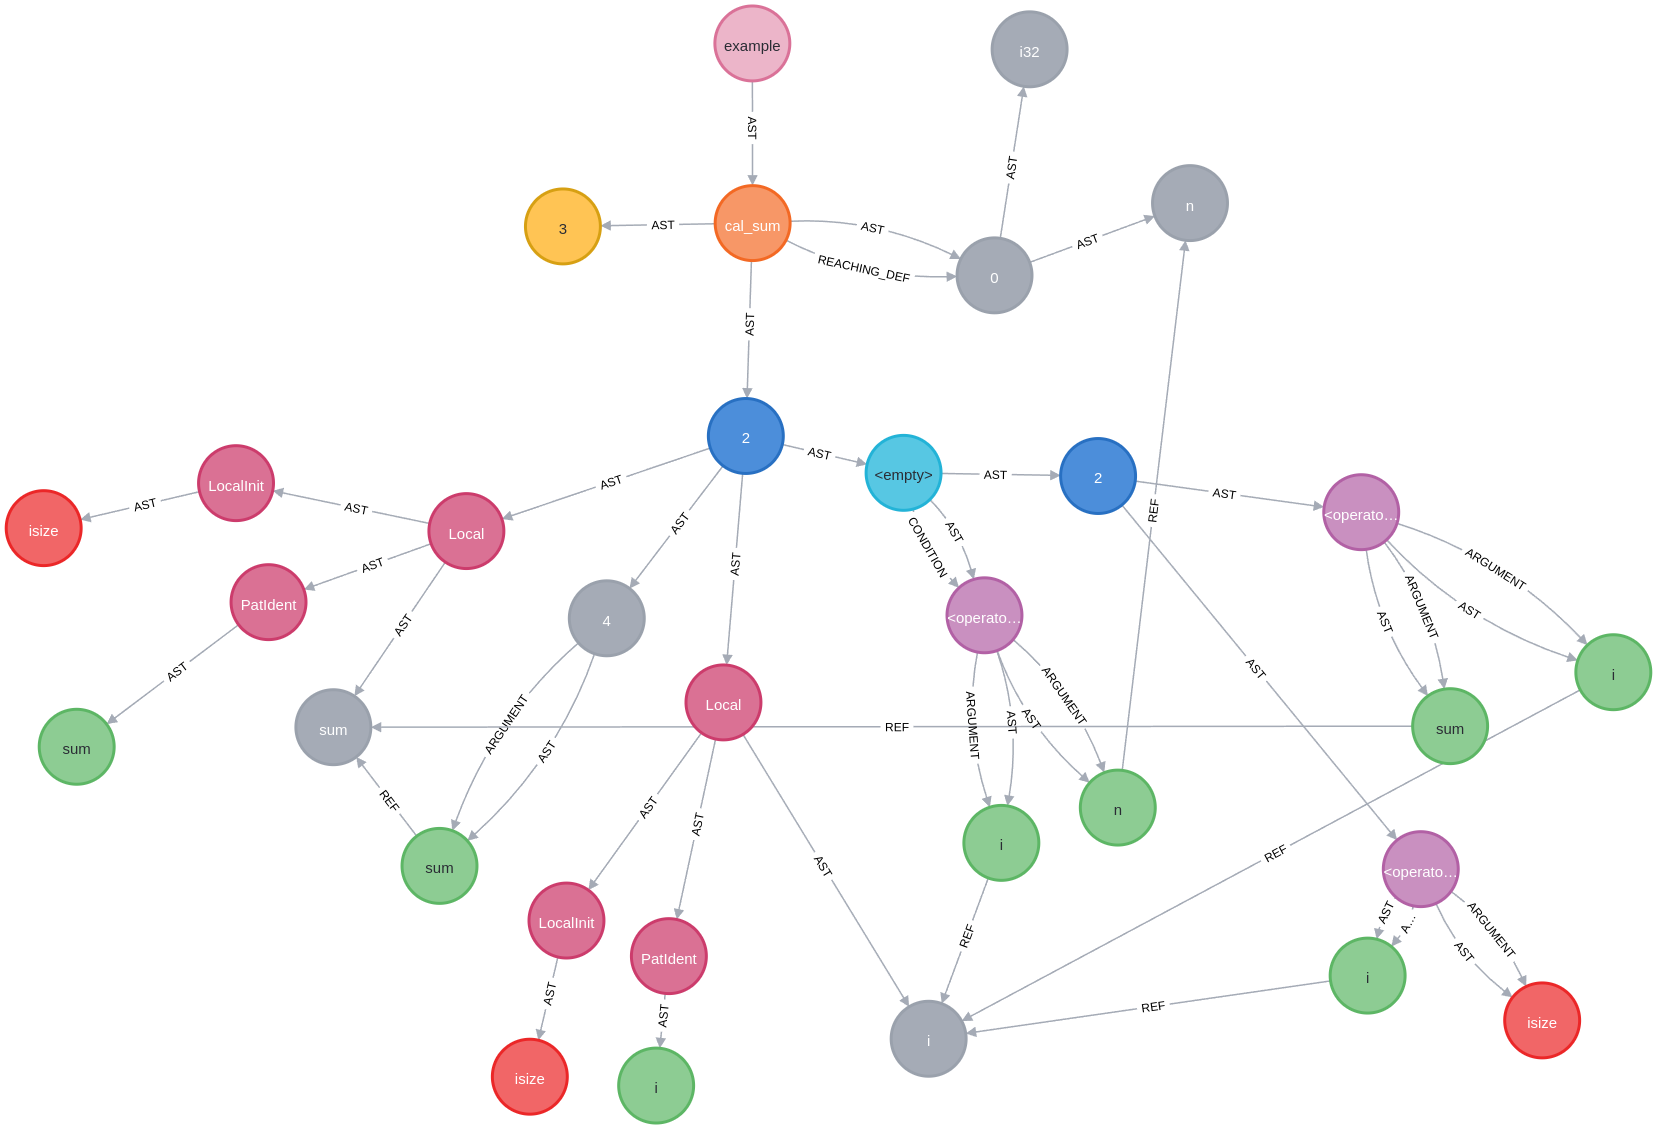
\includegraphics[width=1\columnwidth]{figures/c2/c2_cpg.png}
\centering
\caption{Ví dụ đồ thị thuộc tính mã nguồn cho if let}
\label{img:c3_cpg_iflet}
\end{figure}

\subsection{while let}

\begin{itemize}
    \item Tương tự với tính năng if let ở trên thì Rust cũng hỗ trợ luôn việc khai báo biến làm điều kiện cho vòng lặp while. Có thể hiểu là nếu việc pattern matching của vế trái thành công thì sẽ tiếp tục thực hiện vòng lặp, sẽ có 1 biến $i$ mới được khởi tạo đối với mỗi lần lặp. Các mệnh đề trong khối code khi điều kiện thành công của vòng lặp sẽ tham chiếu tới biến $i$ vừa được khai báo thông qua cạnh $REF$ nếu có sử dụng tới
    \item Không chỉ vậy vế phải của điều kiện có thể được gán lại liên tục trong quá trình lặp, nếu vế phải không match với pattern nào thì vòng lặp sẽ kết thúc.
\end{itemize}

\begin{listing}[H]
\begin{minted}[mathescape, breaklines, frame=lines, framesep=2mm, baselinestretch=1.2, fontsize=\footnotesize, linenos]{rust}
fn main() {
    let mut optional = Some(0);

    while let Some(i) = optional {
        if i > 9 {
            println!("Greater than 9, quit!");
            optional = None;
        } else {
            println!("`i` is `{:?}`. Try again.", i);
            optional = Some(i + 1);
        }
    }
}
\end{minted}
\caption{Ví dụ mã nguồn cho while let}
\label{code:c3_fn}
\end{listing}

\subsection{match}

\begin{itemize}
    \item Ngoài việc có thể sử dụng mệnh đề gán biến thành biểu thức điều kiện, tính hướng hàm của Rust còn thể hiện ở tính match, sự kết hợp giữa pattern matching và Algebraic Data Types. Cấu trúc match trong Rust không chỉ kiểm tra giá trị của một biến mà còn có thể kết hợp với các mẫu phức tạp hơn, bao gồm kiểm tra điều kiện, so sánh phạm vi và kiểm tra các kiểu dữ liệu khác nhau. Điều này mang lại cho Rust tính linh hoạt cao hơn so với switch trong C/C++ và Java, vốn chủ yếu dựa trên so sánh giá trị chính xác.
    \item Một điểm khác biệt quan trọng giữa match và switch là tính toàn diện của match. Rust yêu cầu các mẫu trong match phải bao quát tất cả các khả năng có thể xảy ra, nếu không trình biên dịch sẽ báo lỗi. Điều này giúp đảm bảo rằng không có tình huống nào bị bỏ qua, tăng cường độ an toàn và độ tin cậy của mã nguồn. Trong khi đó, switch trong C/C++ và Java không yêu cầu bao quát tất cả các trường hợp, và việc bỏ sót một trường hợp có thể dẫn đến lỗi logic hoặc hành vi không mong muốn.
    \item Thêm vào đó, match trong Rust hỗ trợ "destructuring", cho phép trích xuất và xử lý các thành phần của cấu trúc dữ liệu phức tạp ngay trong quá trình đối chiếu mẫu. Ví dụ, Rust có thể match trên các tuple, enum, hoặc thậm chí là các phần tử của một mảng, trong khi switch của C/C++ và Java thường chỉ giới hạn trong các giá trị nguyên thủy.
\end{itemize}

\begin{listing}[H]
\begin{minted}[mathescape, breaklines, frame=lines, framesep=2mm, baselinestretch=1.2, fontsize=\footnotesize, linenos]{rust}
enum Color {
    Red,
    Blue(u32, u32, u32),
    Green {
      red: u32,
      green: u32,
      blue: u32,
    },
}

fn main() {
    let color = Color::Blue(0, 0, 255);

    match color {
        Color::Red =>
            println!("The color is Red!")
        Color::Blue(r, g, b) =>
            println!("Red: {}, green: {}, and blue: {}!", r, g, b)
        Color::Green {red, green, blue} =>
            println!(
              "Red: {}, green: {}, and blue: {}!",
              red, green, blue
            ),
    }
}
\end{minted}
\caption{Ví dụ mã nguồn cho match, pattern matching}
\label{code:c3_letelse}
\end{listing}

\subsection{lifetime}

\begin{itemize}
    \item Nói kĩ lại cơ chế của lifetime, cái nào sống lâu hơn cái nào, borrow checker, được kiểm tra vào lúc compile time
    \item Để đáp ứng được tính năng lifetime độc đáo, quan hệ giữa các biến reference có lifetime quan hệ với biến khác. Đồ thị CPG có làm thêm 3 loại node mới là Lifetime, Lifetime Parameter, Lifetime Argument và 1 cạnh $OUT\_LIVE$
    \item Cạnh $OUT\_LIVE$ cực kỳ quan trọng và là điểm chỉnh sửa đặc tả và chỉnh sửa Joern Backend để hỗ trợ lifetime. Cạnh này biểu diễn một biến reference có lifetime quan hệ với biến khác, nếu biến reference này sống lâu hơn biến khác thì cạnh này sẽ chỉ từ biến reference tới biến khác. Các biến reference này sẽ được gán lifetime thông qua cú pháp 'a, 'b, 'c, ...
    \item Nếu các biến cùng đánh dấu lifetime 'a thì sẽ có cạnh $OUT\_LIVE$ tới 'a đó, nếu biến reference này sống lâu hơn biến khác thì cạnh này sẽ chỉ từ biến reference tới biến khác. Đồng thời cũng có thể gán lifetime cho các biến reference thông qua cú pháp 'a: 'b, 'b: 'c, ...
    \item Nói về 3 luật Lifetime Ellision trong Rust, nếu có thể suy luận được lifetime thì không cần phải ghi rõ lifetime, nếu không thể suy luận được thì phải ghi rõ lifetime, nếu có nhiều hơn 1 biến reference thì phải ghi rõ lifetime
    \item Ownership, borrow checker và lifetime là 3 thứ làm nên ngôn ngữ Rust, do vậy khi làm CPG phải làm sao hỗ trợ được 3 tính năng này, thể hiện 3 tính năng này 1 cách rõ ràng, đặc biệt là lifetime
\end{itemize}

\begin{listing}[H]
\begin{minted}[mathescape, breaklines, frame=lines, framesep=2mm, baselinestretch=1.2, fontsize=\footnotesize, linenos]{rust}
fn longest<'a>(x: &'a str, y: &'a str) -> &'a str {
    if x.len() > y.len() {
        x
    } else {
        y
    }
}

fn f<'a, 'b, 'c, 'd: 'c>(x: &'a i32, mut y: &'b i32, z: &'c i32)
where
    'a: 'b,
{
    // ...
}

\end{minted}
\caption{Ví dụ mã nguồn cho lifetime annotation}
\label{code:c3_lifetime}
\end{listing}

